\chapter{Results}
\label{c:results}

Performance tests were performed in the datasets layed out in Chapter \ref{c:datasets}. These aim to show how the system performs in different environments and subject to a variety of attacks. Five metrics are used to evaluate system performance: False Negative (FN) rate, error rate, precision, recall, and F1-score (see \ref{subsec:performance_metrics}).\par
Values in bold were obtained when using three features as input to the model: average time between packets, entropy, and Hamming distance. The remaining values were obtained using only the average time between packets and Hamming distance.

\section{Car Hacking Dataset}

Tests were made monitoring the IDs 350, 130, 131, 140, 2c2, 2b0, 316, 18f, 43f, and 440. The gear spoofing attack targets the ID 43f, and the RPM gauge spoofing attack targets the ID 316. Results are shown in Table \ref{tab:perf_car_hacking}.\par
When using only two features, the F1-score for both spoofing attacks are above 90\%. However, the occurrence of false positives remains high. Including entropy wields generally better results. Although the rate of false negatives is slightly worse, both precision and F1-score show bigger improvements. The fuzzing attack is harder to detect in both cases.\par
Graphics showing feature behaviour during tests can be seen of Figures \ref{fig:extract_carhacking_dos}, \ref{fig:extract_carhacking_fuzzy}, \ref{fig:extract_carhacking_gear}, and \ref{fig:extract_carhacking_rpm}.

\begin{table}
    \centering
    \begin{tabular}{*{6}{c}}
        \toprule
        \textbf{Data} & \textbf{FN rate} & \textbf{Error rate} & \textbf{Precision} & \textbf{Recall} & \textbf{F1-score}\\
        \midrule
        \multirow{2}{*}{Fuzzing} & 1.597\% & 20.300\% & 66.091\% & 98.403\% & 79.074\%\\
        & \textbf{1.632\%} & \textbf{10.746\%} & \textbf{79.134\%} & \textbf{98.368\%} & \textbf{87.709\%}\\
        \multirow{2}{*}{Gear spoofing} & 0.869\% & 10.470\% & 86.554\% & 99.131\% & 92.416\%\\
        & \textbf{1.062\%} & \textbf{2.910\%} & \textbf{96.698\%} & \textbf{98.938\%} & \textbf{97.799\%}\\
        \multirow{2}{*}{RPM spoofing} & 0.871\% & 10.256\% & 87.106\% & 99.129\% & 92.729\%\\
        & \textbf{0.948\%} & \textbf{2.723\%} & \textbf{96.891\%} & \textbf{99.052\%} & \textbf{98.034\%}\\
        \bottomrule
    \end{tabular}
    \caption{Performance metrics on Car Hacking dataset}
    \label{tab:perf_car_hacking}
\end{table}

\section{IEEE Car Hacking: Attack \& Defense Challenge 2020}

The model was trained by gathering a baseline from the attack-free datasets in the stationary and driving modes, separately. Twelve IDs were monitored in each state (44E, 164, 260, 140, 541, 386, 490, 366, 367, 563, 4CB, 50E for the stationary state and 44E, 164, 130, 140, 3A0, 386, 490, 366, 367, 563, 4CB, 2B0 for the driving state). To test the IDS' performance, the stationary model was executed on the datasets provided for the preliminary and final round of the competition, and the driving model was executed on the dataset provided for the preliminary round (the final round did not include a dataset for the driving state).\par
Test results are present in Table \ref{tab:perf_ieee_challenge}. Results for the stationary final and driving tests are above 90\% in both the precision and F1-score metrics. The IDS, however, did not perform so well in the stationary preliminary test. Adding entropy to the set of features reduces the amount of false positives, at the expense of a small increase in the amount of false negatives. The IDS performs slightly worse in the other two tests. Still, it may be preferable to use the three features.\par
Graphics showing feature behaviour during tests can be seen of Figures \ref{fig:extract_ieee_d}, \ref{fig:extract_ieee_s_s}, and \ref{fig:extract_ieee_s_f}.

\begin{table}
    \centering
    \begin{tabular}{*{6}{c}}
        \toprule
        \textbf{Data} & \textbf{FN rate} & \textbf{Error rate} & \textbf{Precision} & \textbf{Recall} & \textbf{F1-score}\\
        \midrule
        \multirow{2}{*}{Stationary Preliminary} & 0.601\% & 19.242\% & 71.264\% & 99.399\% & 83.013\%\\
        & \textbf{0.701\%} & \textbf{16.635\%} & \textbf{74.232\%} & \textbf{99.299\%} & \textbf{84.955\%}\\
        \multirow{2}{*}{Stationary Final} & 0.403\% & 4.478\% & 93.283\% & 99.597\% & 96.337\%\\
        & \textbf{0.403\%} & \textbf{8.004\%} & \textbf{88.349\%} & \textbf{99.597\%} & \textbf{93.636\%}\\
        \multirow{2}{*}{Driving} & 2.591\% & 1.218\% & 99.412\% & 97.409\% & 98.400\%\\
        & \textbf{3.935\%} & \textbf{2.140\%} & \textbf{98.427\%} & \textbf{96.065\%} & \textbf{97.184\%}\\
        \bottomrule
    \end{tabular}
    \caption{Performance metrics on the IEEE Car Hacking: Attack \& Defense Challenge 2020}
    \label{tab:perf_ieee_challenge}
\end{table}

\section{Automotive Controller Area Network (CAN) Bus Intrusion Dataset v2}

Here, the results the tests performed on the datasets described in \ref{subsec:tue_dataset} are shown in Table \ref{tab:perf_tue}. For both the dataset created from traffic gathered from an Opel Astra and a Renault Clio, the IDS was tested on payload fuzzing, message deletion, and replay attacks. For the Opel Astra, the monitored IDs were 0C9, 1C8, 1E2, 232, 348, 34A, 451, 0F1, 1F3, 1E5, and 1A1. For the Renault Clio, the monitored IDs were 2C6, 186, 18A, 1F6, 211, 217, 214, 218, 4FA, and 090. All monitored IDs include the IDs targeted in the attacks, with the rest chosen at random.\par
The payload fuzzing attack goes unnoticed. This happens because, in this case, the attack consists of the modification of the payload of 10 consecutive messages on a given ID, which does not affect either the entropy or Hamming distance values enough to trigger an alert.\par
Graphics showing feature behaviour during tests can be seen of Figures \ref{fig:extract_tue_opelastra_fuzzing}, \ref{fig:extract_tue_opelastra_deletion}, and \ref{fig:extract_tue_opelastra_replay}.

\begin{table}
    \centering
    \begin{tabular}{*{6}{c}}
        \toprule
        \multicolumn{6}{c}{\textbf{Opel Astra}}\\
        \textbf{Data} & \textbf{FN rate} & \textbf{Error rate} & \textbf{Precision} & \textbf{Recall} & \textbf{F1-score}\\
        \midrule
        \multirow{2}{*}{Payload fuzzing} & 100.000\% & 0.408\% & N/A & 0.000\% & N/A\\
        & \textbf{100.000\%} & \textbf{0.408\%} &  \textbf{N/A} & \textbf{0.000\%} & \textbf{N/A}\\
        \multirow{2}{*}{Message deletion} & 18.750\% & 0.491\% & 100.000\% & 81.250\% & 89.655\%\\
        & \textbf{18.750\%} & \textbf{0.491\%} & \textbf{100.000\%} & \textbf{81.250\%} & \textbf{89.655\%}\\
        \multirow{2}{*}{Replay} & 0.000\% & 0.000\% & 100.000\% & 100.000\% & 100.000\%\\
        & \textbf{0.000\%} & \textbf{0.000\%} & \textbf{100.000\%} & \textbf{100.000\%} & \textbf{100.000\%}\\
        \bottomrule
        \toprule
        \multicolumn{6}{c}{\textbf{Renault Clio}}\\
        \textbf{Data} & \textbf{FN rate} & \textbf{Error rate} & \textbf{Precision} & \textbf{Recall} & \textbf{F1-score}\\
        \midrule
        \multirow{2}{*}{Payload fuzzing} & 100.000\% & 2.800\% & 0.000\% & 0.000\% & N/A\\
        & \textbf{100.000\%} & \textbf{2.800\%} & \textbf{0.000\%} & \textbf{0.000\%} & \textbf{N/A}\\
        \multirow{2}{*}{Message deletion} & 27.273\% & 3.629\% & 100.000\% & 72.727\% & 84.746\%\\
        & \textbf{27.273\%} & \textbf{3.629\%} & \textbf{100.000\%} & \textbf{72.727\%} & \textbf{84.211\%}\\
        \multirow{2}{*}{Replay} & 0.000\% & 0.000\% & 100.000\% & 100.000\% & 100.000\%\\
        & \textbf{0.000\%} & \textbf{0.000\%} & \textbf{100.000\%} & \textbf{100.000\%} & \textbf{100.000\%}\\
        \bottomrule
    \end{tabular}
    \caption{Performance metrics on the Automotive Controller Area Network (CAN) Bus Intrusion Dataset v2}
    \label{tab:perf_tue}
\end{table}

\section{CrySyS Lab}

Table \ref{tab:perf_crysys} shows the results of the tests performed on the CrySyS Lab dataset and the generated modification attacks, as described in \ref{sec:dataset_crysys}. Tests were made monitoring 10 IDs (110, 120, 140, 180, 1A0, 280, 290, 295, 300, and 301) and only the attacked ID (120).

\begin{table}
    \centering
    \begin{tabular}{*{6}{c}}
        \toprule 
        \multicolumn{6}{c}{\textbf{Monitoring 10 IDs}}\\
        \midrule
        \textbf{Attack} & \textbf{FN rate} & \textbf{Error rate} & \textbf{Precision} & \textbf{Recall} & \textbf{F1-score}\\
        \midrule
        \multirow{2}{*}{Constant value} & 100.000\% & 40.451\% & 0.000\% & 0.000\% & N/A\\
        & \textbf{100.000\%} & \textbf{40.451\%} & \textbf{0.000\%} & \textbf{0.000\%} & \textbf{N/A}\\
        \multirow{2}{*}{Random value} & 8.992\% & 3.687\% & 99.851\% & 91.008\% & 95.225\%\\
        & \textbf{8.311\%} & \textbf{3.357\%} & \textbf{100.000\%} & \textbf{91.689\%} & \textbf{95.665\%}\\
        \multirow{2}{*}{Adding an increasing value} & 94.959\% & 38.415\% & 97.368\% & 5.051\% & 9.585\%\\
        & \textbf{96.185\%} & \textbf{38.855\%} & \textbf{100.000\%} & \textbf{3.815\%} & \textbf{7.349\%}\\
        \multirow{2}{*}{Decreasing value} & 100.000\% & 40.396\% & N/A & 0.000\% & N/A\\
        & \textbf{100.000\%} & \textbf{40.396\%} & \textbf{N/A} & \textbf{0.000\%} & \textbf{N/A}\\
        \multirow{2}{*}{Delta of 1000} & 99.728\% & 40.341\% & 66.667\% & 0.272\% & 0.543\%\\
        & \textbf{99.864\%} & \textbf{40.341\%} & \textbf{100.000\%} & \textbf{0.136\%} & \textbf{0.272\%}\\
        \bottomrule
        \toprule
        \multicolumn{6}{c}{\textbf{Monitoring 1 ID}}\\
        \midrule
        \textbf{Attack} & \textbf{FN rate} & \textbf{Error rate} & \textbf{Precision} & \textbf{Recall} & \textbf{F1-score}\\
        \midrule
        \multirow{2}{*}{Constant value} & 4.511\% & 1.911\% & 100.000\% & 95.489\% & 97.692\\
        & \textbf{5.263\%} & \textbf{2.229\%} & \textbf{100.000\%} & \textbf{94.737\%} & \textbf{97.297}\\
        \multirow{2}{*}{Random value} & 1.504\% & 0.637\% & 100.000\% & 98.496\% & 99.242\%\\
        & \textbf{0.752\%} & \textbf{0.318\%} & \textbf{100.000\%} & \textbf{99.248\%} & \textbf{99.623\%}\\
        \multirow{2}{*}{Adding an increasing value} & 38.346\% & 16.242\% & 100.000\% & 61.654\% & 76.279\%\\
        & \textbf{24.812\%} & \textbf{10.510\%} & \textbf{100.000\%} & \textbf{75.188\%} & \textbf{85.837\%}\\
        \multirow{2}{*}{Decreasing value} & 100.000\% & 42.357\% & N/A & 0.000\% & N/A\\
        & \textbf{100.000\%} & \textbf{42.357\%} & \textbf{N/A} & \textbf{0.000\%} & \textbf{N/A}\\
        \multirow{2}{*}{Delta of 1000} & 100.000\% & 42.357\% & N/A & 0.000\% & N/A\\
        & \textbf{100.000\%} & \textbf{42.357\%} & \textbf{N/A} & \textbf{0.000\%} & \textbf{N/A}\\
        \bottomrule
    \end{tabular}
    \caption{Performance metrics on the CrySyS Lab datasets}
    \label{tab:perf_crysys}
\end{table}

\section{CES}

The \gls{ids} was trained with the attack-free dataset monitoring the IDs A0, A1, AB, CA, DE, F1, F3, F9, FA, 145, 231, 29D, and 510. Since this dataset is unlabelled, performance metrics, like precision, cannot be used. Instead, Figures \ref{fig:ces_fuzzy} and \ref{fig:ces_spoofing} shows how feature values behave during the fuzzing and spoofing attacks, respectively.\par
In the case of the fuzzing attack, since packets were inserted at a rather slow rate (200ms), the average time between packets, shown in Figure \ref{subfig:ces_fuzzy_avgtime}, does not behave abnormally. Network entropy also remained largely unchanged (Figure \ref{subfig:ces_fuzzy_entropy}). In Figure \ref{subfig:ces_fuzzy_hammingdist}, which shows Hamming distance values, two identifiable spikes corresponding to the two instances of the attack can be seen.\par
As for the spoofing attack, analysis of packet frequency (Figure \ref{subfig:ces_spoofing_avgtime}) does not show any anomalies given the slow rate at which the packets were inserted. Entropy, which can be seen in Figure \ref{subfig:ces_spoofing_entropy}, was also not altered. Hamming distance, however, became anomalous during the two instances of the attack represented by the spikes in Figure \ref{subfig:ces_spoofing_hammingdist}.

\begin{figure}
    \centering
    \begin{subfigure}[b]{.6\linewidth}
        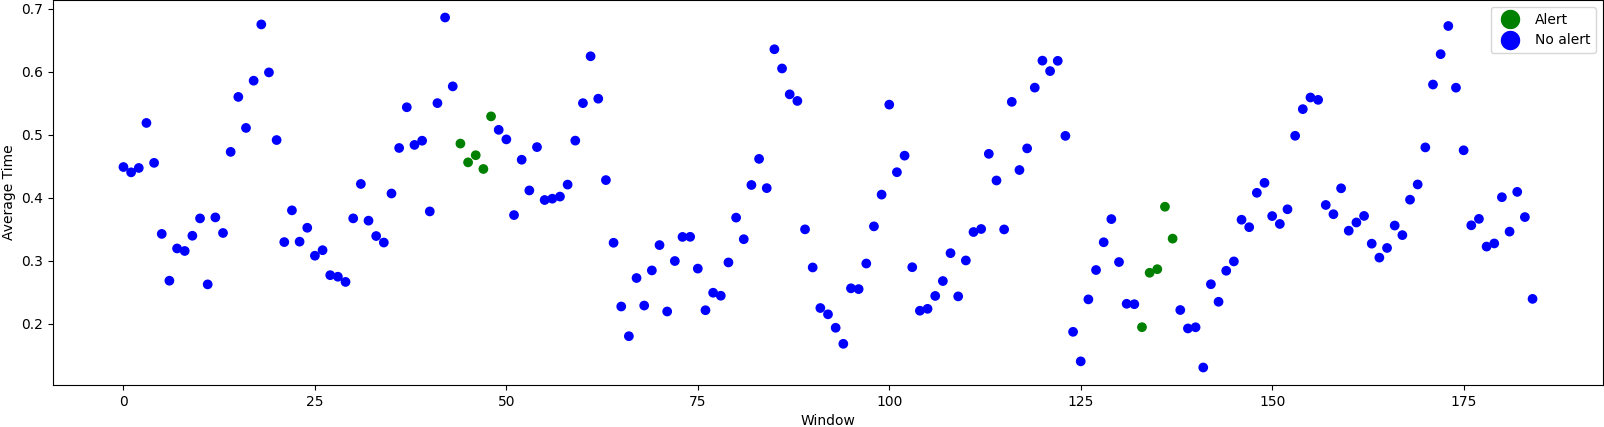
\includegraphics[width = \linewidth]{img/parts/app/tests/ces/fuzzy/AvgTime.png}
        \caption{Average time between packets}
        \label{subfig:ces_fuzzy_avgtime}
    \end{subfigure}
    \begin{subfigure}[b]{.6\linewidth}
        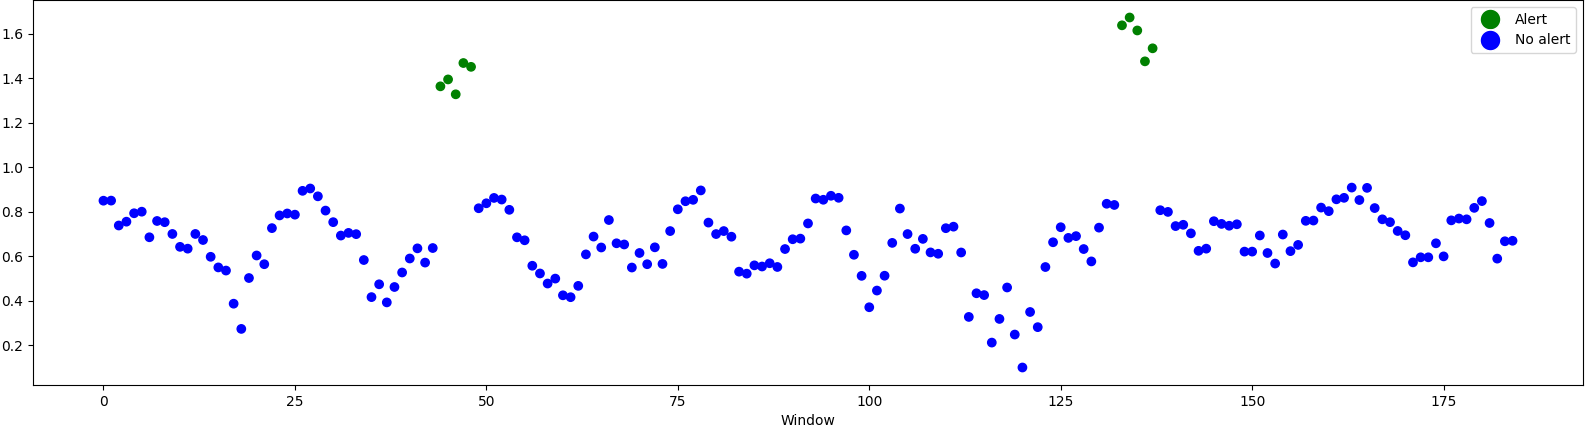
\includegraphics[width = \linewidth]{img/parts/app/tests/ces/fuzzy/HammingDist.png}
        \caption{Hamming distance}
        \label{subfig:ces_fuzzy_hammingdist}
    \end{subfigure}
    \begin{subfigure}[b]{.6\linewidth}
        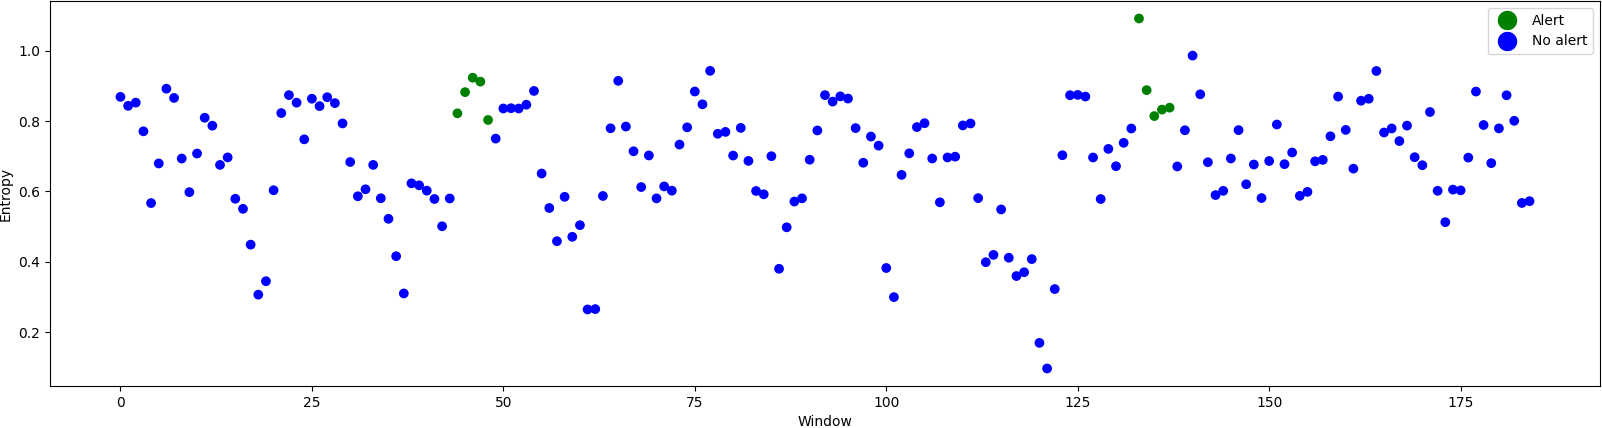
\includegraphics[width = \linewidth]{img/parts/app/tests/ces/fuzzy/Entropy.png}
        \caption{Entropy}
        \label{subfig:ces_fuzzy_entropy}
    \end{subfigure}
    \caption{Features extracted from the fuzzing attack present in the CES dataset}
    \label{fig:ces_fuzzy}
\end{figure}

\begin{figure}
    \centering
    \begin{subfigure}[b]{.6\linewidth}
        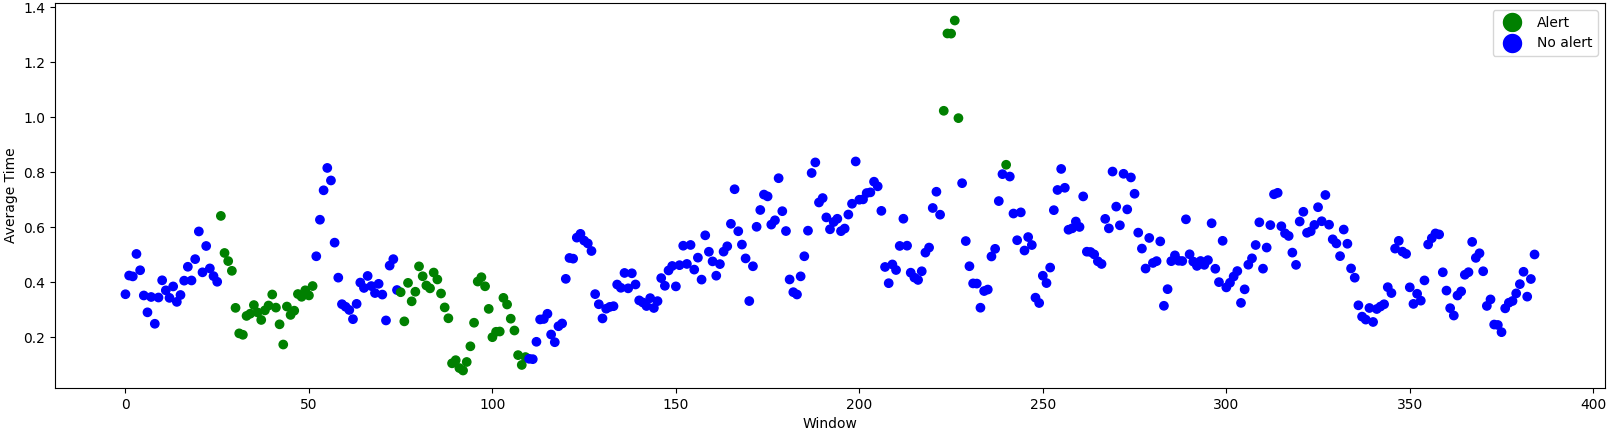
\includegraphics[width = \linewidth]{img/parts/app/tests/ces/spoofing/AvgTime.png}
        \caption{Average time between packets}
        \label{subfig:ces_spoofing_avgtime}
    \end{subfigure}
    \begin{subfigure}[b]{.6\linewidth}
        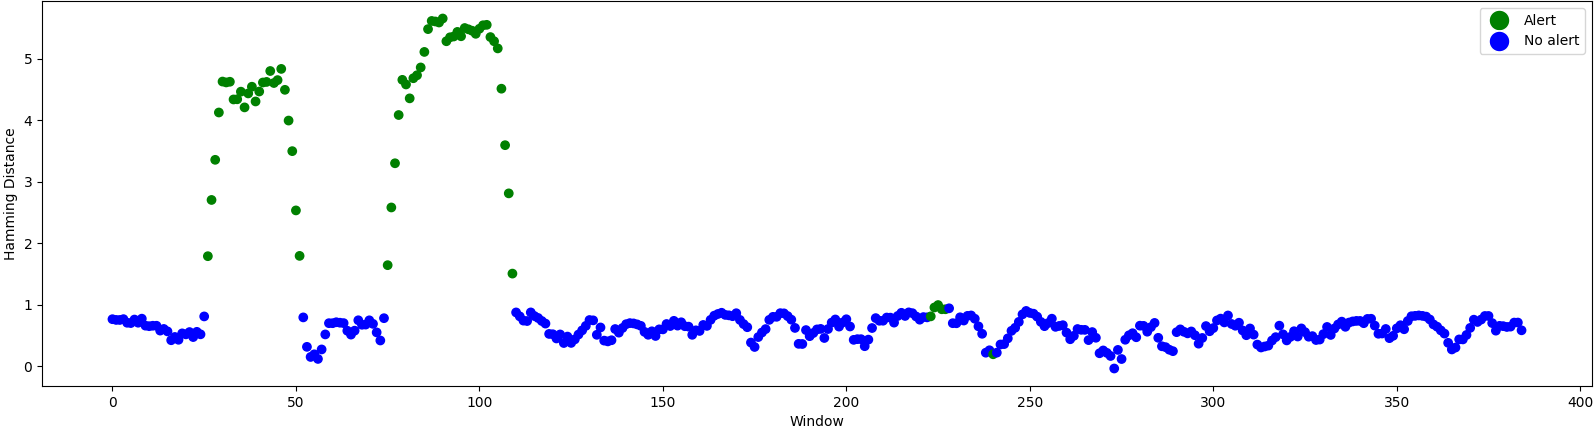
\includegraphics[width = \linewidth]{img/parts/app/tests/ces/spoofing/HammingDist.png}
        \caption{Hamming distance}
        \label{subfig:ces_spoofing_hammingdist}
    \end{subfigure}
    \begin{subfigure}[b]{.6\linewidth}
        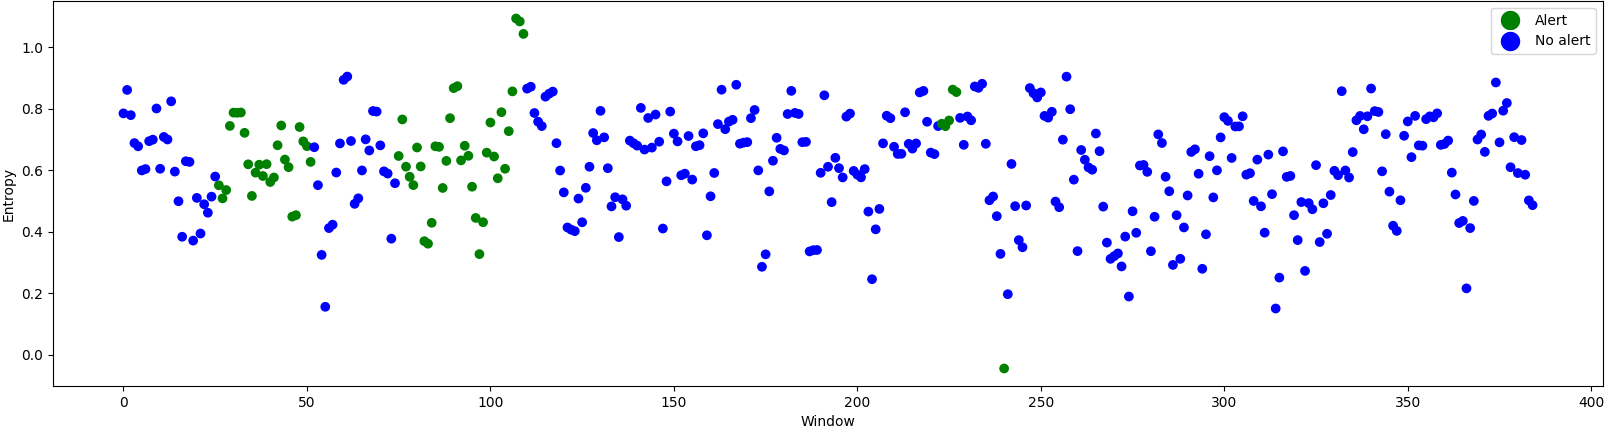
\includegraphics[width = \linewidth]{img/parts/app/tests/ces/spoofing/Entropy.png}
        \caption{Entropy}
        \label{subfig:ces_spoofing_entropy}
    \end{subfigure}
    \caption{Features extracted from the spoofing attack present in the CES dataset}
    \label{fig:ces_spoofing}
\end{figure}